\section*{4.4 特征分解与对角化}
\addcontentsline{toc}{section}{4.4 特征分解与对角化}
\label{sec:4.4}

\emph{对角矩阵（diagonal matrix）} 是指所有非主对角线元素均为零的矩阵，即它们具有如下形式：

\begin{equation}
\boldsymbol{D} = \begin{bmatrix} c_1 & \cdots & 0 \\ \vdots & \ddots & \vdots \\ 0 & \cdots & c_n \end{bmatrix}
\tag{4.49}\label{eq:4-49}
\end{equation}

对角矩阵允许我们快速计算行列式、幂以及逆矩阵。其行列式是对角线上各元素的乘积，矩阵的幂 $ \boldsymbol{D}^k $ 是通过将每个对角线元素取 $ k $ 次幂得到的，而当对角线元素均非零时，其逆矩阵 $ \boldsymbol{D}^{-1} $ 的对角线元素即为原对角线元素的倒数。在本节中，我们将讨论如何将矩阵转换为对角形式。这是我们在第 2.7.2 节中讨论的基变换以及第 4.2 节中讨论的特征值的一个重要应用。

回顾一下，如果存在可逆矩阵 $ \boldsymbol{P} $ 使得 $ \boldsymbol{D} = \boldsymbol{P}^{-1} \boldsymbol{A} \boldsymbol{P} $，则称两个矩阵 $ \boldsymbol{A}, \boldsymbol{D} $ 是相似的（定义 2.22）。更具体地说，我们将研究与对角矩阵 $ \boldsymbol{D} $ 相似的矩阵 $ \boldsymbol{A} $，其中 $ \boldsymbol{D} $ 的对角线上包含 $ \boldsymbol{A} $ 的特征值。

\textbf{定义 4.19}（可对角化 / Diagonalizable）。如果方阵 $ \boldsymbol{A} \in \mathbb{R}^{n \times n} $ 与某个对角矩阵相似，即存在可逆矩阵 $ \boldsymbol{P} \in \mathbb{R}^{n \times n} $ 使得 $ \boldsymbol{D} = \boldsymbol{P}^{-1} \boldsymbol{A} \boldsymbol{P} $，则称 $ \boldsymbol{A} $ 是 \emph{可对角化的（diagonalizable）} 。

在下文中，我们将看到对矩阵 $ \boldsymbol{A} \in \mathbb{R}^{n \times n} $ 进行对角化是在另一组基下表示同一线性映射的一种方式（参见第 2.6.1 节），并且事实表明这组基由 $ \boldsymbol{A} $ 的特征向量组成。

设 $ \boldsymbol{A} \in \mathbb{R}^{n \times n} $，设 $ \lambda_1, \ldots, \lambda_n $ 是一组标量，并设 $ \boldsymbol{p}_1, \ldots, \boldsymbol{p}_n $ 是 $ \mathbb{R}^n $ 中的一组向量。我们定义 $ \boldsymbol{P} := [\boldsymbol{p}_1, \ldots, \boldsymbol{p}_n] $，并设 $ \boldsymbol{D} \in \mathbb{R}^{n \times n} $ 是对角线元素为 $ \lambda_1, \ldots, \lambda_n $ 的对角矩阵。那么我们可以证明：

\begin{equation}
\boldsymbol{A} \boldsymbol{P} = \boldsymbol{P} \boldsymbol{D}
\tag{4.50}\label{eq:4-50}
\end{equation}

当且仅当 $ \lambda_1, \ldots, \lambda_n $ 是 $ \boldsymbol{A} $ 的特征值，且 $ \boldsymbol{p}_1, \ldots, \boldsymbol{p}_n $ 是 $ \boldsymbol{A} $ 对应的特征向量。

我们可以看到该命题成立，因为：

\begin{equation}
\boldsymbol{A} \boldsymbol{P} = \boldsymbol{A} [\boldsymbol{p}_1, \ldots, \boldsymbol{p}_n] = [\boldsymbol{A} \boldsymbol{p}_1, \ldots, \boldsymbol{A} \boldsymbol{p}_n]
\tag{4.51}\label{eq:4-51}
\end{equation}

\begin{equation}
\begin{adjustbox}{max width=\linewidth}
\boldsymbol{P} \boldsymbol{D} = [\boldsymbol{p}_1, \ldots, \boldsymbol{p}_n] \begin{bmatrix} \lambda_1 & & 0 \\ & \ddots & \\ 0 & & \lambda_n \end{bmatrix} = [\lambda_1 \boldsymbol{p}_1, \ldots, \lambda_n \boldsymbol{p}_n]
\end{adjustbox}
\tag{4.52}\label{eq:4-52}
\end{equation}

因此，式~\eqref{eq:4-50} 意味着：

\begin{equation}
\boldsymbol{A} \boldsymbol{p}_1 = \lambda_1 \boldsymbol{p}_1
\tag{4.53}\label{eq:4-53}
\end{equation}

\begin{equation*}
\vdots
\end{equation*}

\begin{equation}
\boldsymbol{A} \boldsymbol{p}_n = \lambda_n \boldsymbol{p}_n
\tag{4.54}\label{eq:4-54}
\end{equation}

所以，$ \boldsymbol{P} $ 的各列必须是 $ \boldsymbol{A} $ 的特征向量。

我们对对角化的定义要求 $ \boldsymbol{P} \in \mathbb{R}^{n \times n} $ 是可逆的，即 $ \boldsymbol{P} $ 具有满秩（定理 4.3）。这要求我们拥有 $ n $ 个线性无关的特征向量 $ \boldsymbol{p}_1, \ldots, \boldsymbol{p}_n $，即 $ \boldsymbol{p}_i $ 构成 $ \mathbb{R}^n $ 的一组基。

\textbf{定理 4.20}（特征分解 / Eigendecomposition）。方阵 $ \boldsymbol{A} \in \mathbb{R}^{n \times n} $ 可以分解为

\begin{equation}
\boldsymbol{A} = \boldsymbol{P} \boldsymbol{D} \boldsymbol{P}^{-1}
\tag{4.55}\label{eq:4-55}
\end{equation}

其中 $ \boldsymbol{P} \in \mathbb{R}^{n \times n} $，且 $ \boldsymbol{D} $ 是对角线元素为 $ \boldsymbol{A} $ 的特征值的对角矩阵，当且仅当 $ \boldsymbol{A} $ 的特征向量构成 $ \mathbb{R}^n $ 的一组基。


\begin{figure}[H]
\centering
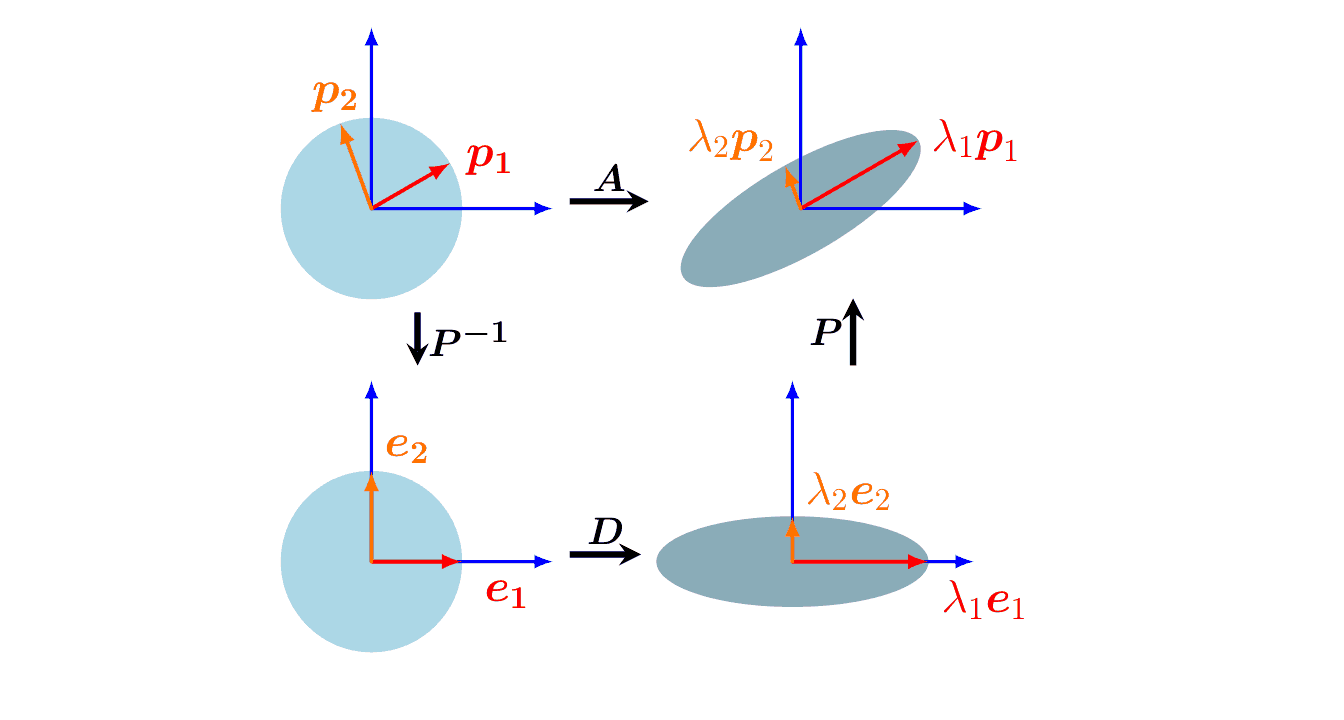
\includegraphics[width=0.92\textwidth,keepaspectratio]{docs/images/Figure4.7.png}
\caption*{\refstepcounter{figcounter}\label{fig:4-7}图~\thefigcounter 将特征分解理解为一系列连续变换的几何直观。左上到左下：P⁻¹ 执行基变换（此处在 R² 中绘制，表示为类似旋转的操作），将特征向量映射到标准基。左下到右下：D 沿着重新映射的正交特征向量进行缩放，此处由圆拉伸为椭圆来表示。右下到右上：P 撤销基变换（表示为反向旋转）并恢复原始坐标系。}
\end{figure}


定理 4.20 表明只有非亏损矩阵才可以对角化，并且 $ \boldsymbol{P} $ 的各列是 $ \boldsymbol{A} $ 的 $ n $ 个特征向量。对于对称矩阵，我们可以在特征值分解方面获得更强的结论。

\textbf{定理 4.21}。对称矩阵 $ \boldsymbol{S} \in \mathbb{R}^{n \times n} $ 总是可以对角化的。

定理 4.21 直接由谱定理（定理 4.15）得出。此外，谱定理指出我们可以找到由 $ \mathbb{R}^n $ 的特征向量构成的标准正交基（ONB）。这使得 $ \boldsymbol{P} $ 成为正交矩阵，从而 $ \boldsymbol{D} = \boldsymbol{P}^\top \boldsymbol{A} \boldsymbol{P} $。

\emph{备注} 。矩阵的若尔当标准形（Jordan normal form）提供了一种适用于亏损矩阵的分解方法（Lang, 1987），但这超出了本书的讨论范围。♦

\section*{特征分解的几何直观}
\addcontentsline{toc}{subsection}{特征分解的几何直观}

我们可以将矩阵的特征分解解释如下（亦见图~\ref{fig:4-7}）：设 $ \boldsymbol{A} $ 为关于标准基的线性映射的变换矩阵。$ \boldsymbol{P}^{-1} $ 执行从标准基到特征基的基变换。这把特征向量 $ \boldsymbol{p}_i $（图~\ref{fig:4-7} 中的红色和橙色箭头）映射到标准基向量 $ \boldsymbol{e}_i $ 上。然后，对角矩阵 $ \boldsymbol{D} $ 沿着这些坐标轴按特征值 $ \lambda_i $ 对向量进行缩放。最后，$ \boldsymbol{P} $ 将这些缩放后的向量变换回标准/规范坐标系，得到 $ \lambda_i \boldsymbol{p}_i $。

\begin{notebox}
\textbf{例 4.11（特征分解）}
\end{notebox}

\begin{notebox}
我们来计算矩阵

\begin{equation*}
\boldsymbol{A} = \begin{bmatrix} 2 & 1 \\ 1 & 2 \end{bmatrix}
\end{equation*}

的特征分解。
\end{notebox}

\begin{notebox}
\textbf{步骤 1：计算特征值和特征向量。} $ \boldsymbol{A} $ 的特征多项式为：

\begin{equation}
\det(\boldsymbol{A} - \lambda \boldsymbol{I}) = \det\begin{bmatrix} 2 - \lambda & 1 \\ 1 & 2 - \lambda \end{bmatrix}
\tag{4.56a}\label{eq:4-56a}
\end{equation}

\begin{equation}
= (2 - \lambda)^2 - 1 = \lambda^2 - 4\lambda + 3 = (\lambda - 3)(\lambda - 1)
\tag{4.56b}\label{eq:4-56b}
\end{equation}

因此，$ \boldsymbol{A} $ 的特征值为 $ \lambda_1 = 1 $ 和 $ \lambda_2 = 3 $（特征多项式的根），对应的（归一化）特征向量通过下式求得：

\begin{equation}
\begin{bmatrix} 2 & 1 \\ 1 & 2 \end{bmatrix} \boldsymbol{p}_1 = 1 \boldsymbol{p}_1, \quad \begin{bmatrix} 2 & 1 \\ 1 & 2 \end{bmatrix} \boldsymbol{p}_2 = 3 \boldsymbol{p}_2
\tag{4.57}\label{eq:4-57}
\end{equation}

由此解得：

\begin{equation}
\boldsymbol{p}_1 = \frac{1}{\sqrt{2}} \begin{bmatrix} 1 \\ -1 \end{bmatrix}, \quad \boldsymbol{p}_2 = \frac{1}{\sqrt{2}} \begin{bmatrix} 1 \\ 1 \end{bmatrix}
\tag{4.58}\label{eq:4-58}
\end{equation}
\end{notebox}

\begin{notebox}
\textbf{步骤 2：检验存在性。} 特征向量 $ \boldsymbol{p}_1, \boldsymbol{p}_2 $ 构成 $ \mathbb{R}^2 $ 的一组基。因此，$ \boldsymbol{A} $ 可以对角化。
\end{notebox}

\begin{notebox}
\textbf{步骤 3：构造对角化 $ \boldsymbol{A} $ 的矩阵 $ \boldsymbol{P} $。} 我们将 $ \boldsymbol{A} $ 的特征向量组合在 $ \boldsymbol{P} $ 中，使得：

\begin{equation}
\boldsymbol{P} = [\boldsymbol{p}_1, \boldsymbol{p}_2] = \frac{1}{\sqrt{2}} \begin{bmatrix} 1 & 1 \\ -1 & 1 \end{bmatrix}
\tag{4.59}\label{eq:4-59}
\end{equation}

接着我们得到：

\begin{equation}
\boldsymbol{P}^{-1} \boldsymbol{A} \boldsymbol{P} = \begin{bmatrix} 1 & 0 \\ 0 & 3 \end{bmatrix} = \boldsymbol{D}
\tag{4.60}\label{eq:4-60}
\end{equation}

等价地，我们得到（利用在本例中特征向量 $ \boldsymbol{p}_1 $ 和 $ \boldsymbol{p}_2 $ 构成一组标准正交基，从而 $ \boldsymbol{P}^{-1} = \boldsymbol{P}^\top $）：

\begin{equation}
\begin{adjustbox}{max width=\linewidth}
\underbrace{\begin{bmatrix} 2 & 1 \\ 1 & 2 \end{bmatrix}}_{\boldsymbol{A}} = \underbrace{\frac{1}{\sqrt{2}} \begin{bmatrix} 1 & 1 \\ -1 & 1 \end{bmatrix}}_{\boldsymbol{P}} \underbrace{\begin{bmatrix} 1 & 0 \\ 0 & 3 \end{bmatrix}}_{\boldsymbol{D}} \underbrace{\frac{1}{\sqrt{2}} \begin{bmatrix} 1 & -1 \\ 1 & 1 \end{bmatrix}}_{\boldsymbol{P}^\top}
\end{adjustbox}
\tag{4.61}\label{eq:4-61}
\end{equation}
\end{notebox}

对角矩阵 $ \boldsymbol{D} $ 可以非常高效地进行求幂运算。因此，我们可以通过特征值分解（如果存在）来计算矩阵 $ \boldsymbol{A} \in \mathbb{R}^{n \times n} $ 的幂，使得：

\begin{equation}
\boldsymbol{A}^k = (\boldsymbol{P} \boldsymbol{D} \boldsymbol{P}^{-1})^k = \boldsymbol{P} \boldsymbol{D}^k \boldsymbol{P}^{-1}
\tag{4.62}\label{eq:4-62}
\end{equation}

计算 $ \boldsymbol{D}^k $ 是高效的，因为我们只需对每个对角线元素分别进行该操作。

假设特征分解 $ \boldsymbol{A} = \boldsymbol{P} \boldsymbol{D} \boldsymbol{P}^{-1} $ 存在。那么：

\begin{equation}
\det(\boldsymbol{A}) = \det(\boldsymbol{P} \boldsymbol{D} \boldsymbol{P}^{-1}) = \det(\boldsymbol{P}) \det(\boldsymbol{D}) \det(\boldsymbol{P}^{-1})
\tag{4.63a}\label{eq:4-63a}
\end{equation}

\begin{equation}
= \det(\boldsymbol{D}) = \prod_{i=1}^n d_{ii}
\tag{4.63b}\label{eq:4-63b}
\end{equation}

这使得我们可以高效地计算 $ \boldsymbol{A} $ 的行列式。

特征值分解要求矩阵是方阵。若能对一般矩阵执行分解将会非常有用。在下一节中，我们将介绍一种更一般的矩阵分解技术：奇异值分解。
